
\documentclass{llncs}

\usepackage{llncsdoc}

\usepackage{tikz}
\usetikzlibrary{positioning,automata}


\usepackage{graphicx}
\usepackage{amsmath}
\usepackage{xspace}
\usepackage{footnote}
\usepackage{cite}
\usepackage{amsfonts}
\usepackage{float}
%\usepackage{natbib}
\usepackage{hhline}
\usepackage{multirow}
\usepackage{amssymb}
\usepackage[hyphens]{url}
\usepackage[colorlinks,linkcolor=blue,citecolor=blue,urlcolor=blue]{hyperref}
\usepackage[hyphenbreaks]{breakurl}
\usepackage{xcolor}
\usepackage{listings}
\usepackage{mathpartir}
\usepackage{caption}
\usepackage{subcaption}


\usetikzlibrary{calc}
\usetikzlibrary{automata}
\usetikzlibrary{backgrounds}
\usetikzlibrary{decorations.pathreplacing}
\usetikzlibrary{shapes,arrows}
\usetikzlibrary{positioning}
\usetikzlibrary{shadows}
\usetikzlibrary{circuits.logic.US}


\newcommand{\fullNN}{\ensuremath{N(accel,break,rpm,speed,gear)}}
\newcommand{\fullNNAtk}{\ensuremath{N(accel,break,rpm,speed_{ATK},gear)}}
\newcommand{\isAccel}{\ensuremath{A(accel,brake)}}
\newcommand{\speedGear}{\ensuremath{R(rpm,gear)}}
\newcommand{\rpmGear}{\ensuremath{S(speed,gear)}}

\newcommand{\isUnderAttack}{\ensuremath{Atk()}}

\newcommand{\inputSig}[2]{\ensuremath{\sigma_{#1}^{#2}}}
\newcommand{\outputSig}[2]{\ensuremath{\varsigma_{#1}^{#2}}}
\newcommand{\atkBegin}{\ensuremath{a_{0}}}
\newcommand{\atkLength}{\ensuremath{a}}

\newcommand{\nats}{\ensuremath{\mathbb{N}}}
\newcommand{\signal}{\ensuremath{s}}
\newcommand{\from}{\ensuremath{\colon}}
\newcommand{\dtime}{\mbox{\ensuremath{\mathcal{T}\hspace{-2.5pt}\scalebox{0.8}{\ensuremath{\boldsymbol{i}\boldsymbol{m}\boldsymbol{e}}}}}}
\renewcommand{\to}{\ensuremath{\rightarrow}}
\newcommand{\values}{\ensuremath{\mathcal{V}}}
\newcommand{\inputs}{\ensuremath{\mathcal{S}_{I}}}
\newcommand{\outputs}{\ensuremath{\mathcal{S}_{O}}}
\newcommand{\signals}{\ensuremath{\mathcal{S}}}
\newcommand{\bool}{\ensuremath{\mathcal{B}}}
\newcommand{\mealy}{\ensuremath{\mathbb{M}}\xspace}
\newcommand{\cfm}{\ensuremath{\mathcal{M}}\xspace}
\newcommand{\term}{\ensuremath{\tau}}
\newcommand{\fterm}{\ensuremath{\term_{F}}\xspace}
\newcommand{\pterm}{\ensuremath{\term_{P}}\xspace}
\newcommand{\uterm}{\ensuremath{\term_{U}}}
\newcommand{\name}[1]{{\text{\texttt{#1}}}}
\newcommand{\terms}{\ensuremath{\mathcal{T}}\xspace}
\newcommand{\comp}{\ensuremath{\varsigma}\xspace}
\newcommand{\comps}{\ensuremath{\mathcal{C}}}
\newcommand{\init}{\ensuremath{\iota}}
\newcommand{\inits}{\ensuremath{\name{init}_{\name{s}}}\xspace}
\newcommand{\sep}{\ensuremath{\quad | \quad}}
\newcommand{\upd}[2]{\ensuremath{[\,#1 \lhd \, #2\,]}}
\newcommand{\sats}{\ensuremath{\vDash}}
\newcommand{\nsats}{\ensuremath{\nvDash}}
\newcommand{\set}[1]{\ensuremath{\{ #1 \}}}
\newcommand{\eval}{\ensuremath{\eta}\xspace}



\begin{document}

\special{papersize=8.5in,11in}
\setlength{\pdfpageheight}{\paperheight}
\setlength{\pdfpagewidth}{\paperwidth}

% Uncomment one of the following two, if you are not going for the 
% traditional copyright transfer agreement.

%\exclusivelicense                % ACM gets exclusive license to publish, 
                                  % you retain copyright

%\permissiontopublish             % ACM gets nonexclusive license to publish
                                  % (paid open-access papers, 
                                  % short abstracts)

%\titlebanner{banner above paper title}        % These are ignored unless
%\preprintfooter{short description of paper}   % 'preprint' option specified.

\title{Hybrid Automota Reachability for Sensor Spoofing Vulnerability Analysis}

\author{\xspace}
\institute{\xspace}

\maketitle
\begin{abstract}

Neural networks have been leveraged to great effect in the construction of efficient and performant cyber physical systems.
However, this has introduced a problem of legibility - it is difficult to make formal arguments about the behavior of learned systems.
We propose an approach to structured machine learning by leveraging program synthesis.
We synthesize automata from temporal logic specifications, and use the automata as a combination strategy for many smaller neural networks.
We provide a measure of the attack surface of a neural network, and demonstrate that our approach results in safer systems.
As a case study, we run simulate an sensor spoofing attack in a vehicle simulator and measure the time to recovery for our system and a typical monolithic controller.

\end{abstract}

\section{Introduction}

Autonomous vehicles are considered to be one of the most challenging
types of reactive systems currently under development. They need to
interact with a highly reactive environment. Life critical decisions
have to be made instantaneously and need to be executed at the right
point in time. However, even if the intricate task of designing such
systems is conquered, it still needs to be ensured, that the result is
also safe and reliable.



\begin{itemize}

\item explain the rise of functional programming languages, and that 
types provide intuitive reasoning about safety

\item explain that functional languages now also are used for hardware
  (embedded systems people probably don't know about that) (mention
  results like \emph{clash} or \emph{Kansas Lava})

\item for reactive systems, a proper notion of time is necessary,
  motivate on some example (synchronous vs asynchronous, real vs
  discrete), finally lead to FRP

\item motivate FRP (this is the most important part, almost sure that
  nobody of the reviews will know about; go through the very basics,
  remember these are embedded systems people)

\item we provide first example of using FRP to control autonomous
  vehicle, our approach is elegant and simple, which makes it
  resistant against errors. Furthermore it is easily extendable
  without breaking the remaining system.

\end{itemize}


\section{Motivating Example}

We take as a motivating example, the gearing controller component for an autonomous vehicle system.
In a typical scenario, we might build a neural network to control the output of the gear box at every time step based on all relevant sensor data.
We then have a neural network, $\fullNN$, processing inputs (acceleration, braking, speed, rpm, gear) to produce a new (gear) signal.

We can imagine this as a mealy machine with a single state and a single transition, which is always active.

\begin{figure}[h!]
\centering
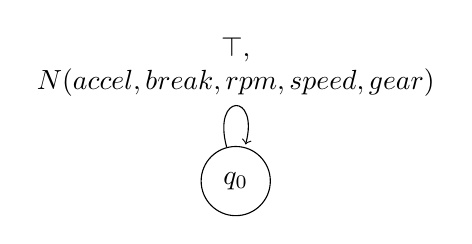
\begin{tikzpicture}[shorten >=1pt,node distance=2.8cm,on grid]
  \node[state]   (q_0)                {$q_0$};
  \path[->] (q_0) 
		  edge [loop above]   node  [above,align=center]         {$\top,$\\$ \fullNN$} ();
\end{tikzpicture}
\caption{A mealy machine of a single monolithic neural network}
\label{fig:full}
\end{figure}

Now assume we have some adversarial actor that takes control of the speed sensor.
Since this network is processing the speed signal at every time step, we cannot have any guarantee of the effect a faulty speed sensor will have on our overall output.

In contrast, imagine we build an automata of neural networks as below.
Here, we have composed three networks; $\isAccel$ for a binary classifier that indicates whether the car is accelerating and the two multiclass classifiers, $\rpmGear$ and $\speedGear$, mapping their inputs to the target gear into which the car should shift (for example gears 1-5).
The mealy machine says that when the car is not accelerating, we should not shift the gear.
It also specifies that when we start to accelerate after a period of slowing down, we should set the gear based on the current speed.
As the car continues to accelerate, the gear should be set based on the rpm of the engine.

\begin{figure}[h!]
\centering
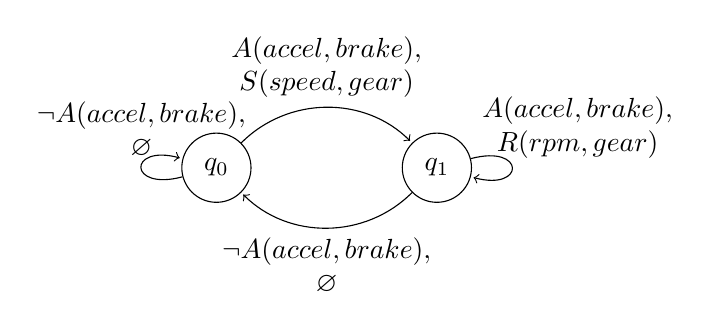
\begin{tikzpicture}[shorten >=1pt,node distance=2.8cm,on grid]
  \node[state]   (q_0)                {$q_0$};
  \node[state] (q_1) [right=of q_0] {$q_1$};
  \path[->] (q_0) 
		  edge [loop left]   node  [above,align=center]         {$\neg \isAccel,$\\$ \varnothing$} ()
		  edge [bend left=45] node [above,align=center] {$\isAccel,$\\$ \rpmGear$} (q_1)
            (q_1) 
		  edge [loop right]   node [above right,xshift=-0.5cm,align=center]        {$\isAccel,$\\$ \speedGear$} ()
		  edge [bend left=45] node [below,align=center] {$\neg \isAccel,$\\$ \varnothing$} (q_0);
\end{tikzpicture}
\caption{A mealy machine of multiple composed neural networks}
\label{fig:components}
\end{figure}

In Fig.~\ref{fig:components}, we clearly see that an attack on the speed sensor is guaranteed to only have an effect on the transition from state $q_0$ to state $q_1$.
Because of this compartmentalization of vulnerability, safety tactics such as trying to detect anomalous values may be employed to greater effect.
In the sequel, we will present a quantitative formalization of the vulnerability of the systems in both Fig.~\ref{fig:full} and Fig.~\ref{fig:components}.


\section{Saftey}

In this section, building off the definition provided in~\cite{DBLP:journals/corr/HuangKWW16}, we provide a formal definition of the vulnerability to advererial input of a mealy machine where the transition actions are neural networks.
We then show how by decomposing a larger neural network into an automata of smaller neural networks, we can reduce the overall vulnerability of the system.
Relying on the structure of the automata connecting the network, we can provide formal proofs activation periods of each individual network and demonstrate that adversarial inputs are less likely to be acted upon within a given time frame.


\section{Parameterized Synthesis}

We show how FRP synthesis can be parameterized over pure function implementations, thereby providing a nice target for combination with machine learning.


\section{Case Study: TORCS}

We use the Haskell bindings to TORCS to synthesize an FRP controller for a autonomous vehicle.
Since our synthesis procedure requires implementations of the pure functions to be complete, we leave those details to machine learning.

\subsection{Specifying a Driver}

\subsection{Optimization}
As a simpler case, we first provide rough implementations of the pure functions, leaving out only the critical values such as target speed and turning radius.
We use stochastic gradient descent to find optmimal values (where the cost is the lap time) to be embedded in the pure functions.


\subsection{Full Synthesis}
In this section we demonstrate how to use a nueral network to generate the low level interpretation of the pure functions to machine learning.
In this way, we still rely on the formalized program synthesis to give us a correct by construction framework for the driver.




\section{Related Work}

TORCS has been proven to provide an expressive framework for the research community~\cite{OnievaPAMP09,conf/cig/CardamoneLL09,conf/cig/MunozGS10}. 
For instance, it has been used for formal verification of platoons~\cite{kamali2016formal}. 
None of these works have used FRP as the language for the controller.


FRP specifically has been proposed as a tool for vehicle control~\cite{kazemi2016,zou2016}, where FRP was extended to prioritize functions for timing constraints. However, due to the lack of a compatible simulator, the vehicle simulation never was implemented. 

FRP has also been used for embedded systems~\cite{helbling2016juniper} and networking~\cite{voellmy2012scalable}.
The FRP networking library took advantage of Haskell's multicore support and significantly outperformed competing tools written in C++ and Java.


To the best of our knowledge this is the first FRP-based vehicle simulator.
Although there are many bindings to various vehicle simulators, these tend to use imperative languages.
For instance, TORCS allows users to directly edit the source code and add a new car in C++.
There are also TORCS bindings for python, java, and matlab, which have been used in the SCRC competition~\cite{SCRC}.

The videogame GTA~\cite{} has also been used to train image recognition software for autonomous vehicles~\cite{}.
While GTA is professionally produced game, which has more attractive graphics and a more advanced physics engine, it has a different set of issues.
First, it is proprietary software not designed for autonomous vehicle research. 
Hence, the ability to build sensor based controllers is more restricted. 
Second, unlike TORCS, which is designed primarily as a vehicle simulator, GTA's physics engine is tuned to maximize entertainment.
Using GTA as a meaningful control simulator would still be valuable work, but we leave this to the future.


\section{Conclusions}

\subsection{Future Work}

Since DFA are equivalent to Recurrent Neural Networks in expressibility, it would be interesting to replace the Mealy machine as a gating network with a RNN.
It is possible that,in practice, the particular structure of the gating network is more powerful than required. 
Instead, just by defining the subnetworks (the experts), this may be sufficient to maintain some safety properties.

In our analysis we have only viewed this problem from a verification perspective. 
An additional complexity is the actual learning rate and effectiveness of such a network structure.
We know that the Mixture of Experts architecture can be used to reduce the training time in general, but so far we have not explored the effect of using a Mealy machine as the gating network on the learning process.
Such an analysis is more well-suited to the machine learning community.


\bibliographystyle{splncs03}
\bibliography{sigproc}

\end{document}


